\documentclass{resume}

\name{Jiangkun QIU}
\address{
    \faPhone~+852 91408309(WA)
    \faEnvelope~\href{mailto://qjk2001@gmail.com}{qjk2001@gmail.com} \faGithub~\href{https://github.com/JakkuSakura/}{JakkuSakura} \faWeixin~JakkuSakura ~~~~~~~
}


\begin{document}

\begin{tikzpicture}[remember picture, overlay] 
    %\node[anchor = north east] at ($(current page.north east)+(-1.3cm,-1.2cm)$) {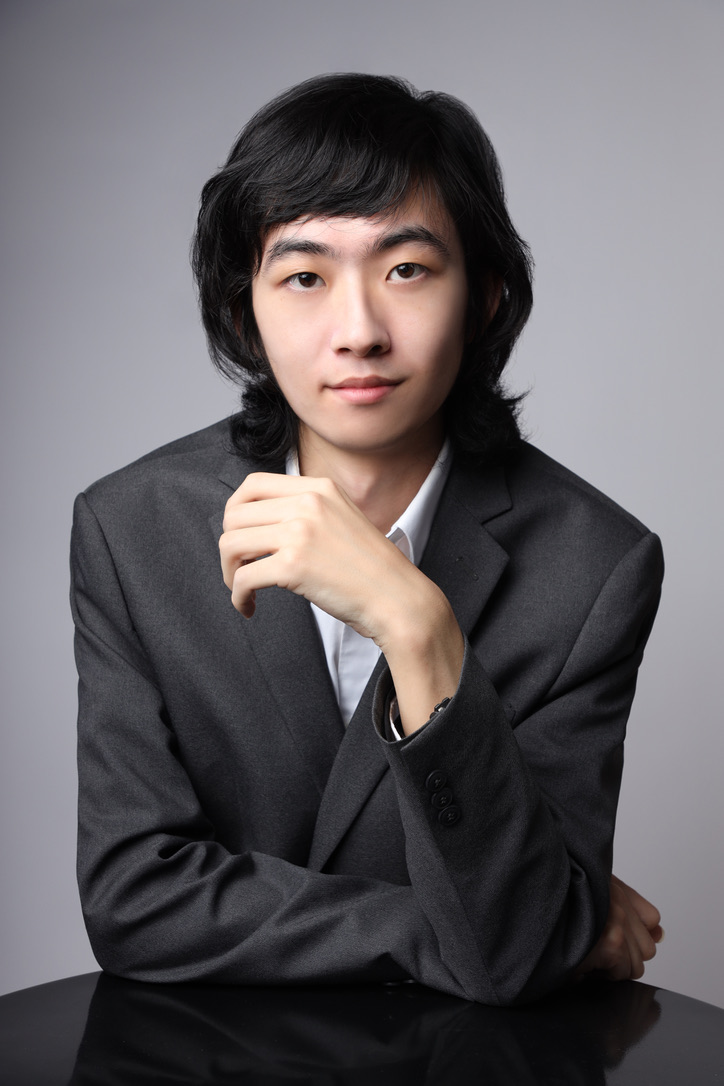
\includegraphics[height=2.5cm]{avatar.jpg}};
\end{tikzpicture}

\begin{rSection}{\faCogs~Skill Set}
    \begin{itemize}
        \itemsep -0.5em
        \item Expertise in Rust for 3 years in High Frequency Trading and web3.
        \item Long history of learning Java, C, C++ since primary school 
        \item Algorithm and Data Structure training and competitions in middle and high school
        \item A wide technical stack, all main stream languages in fields from backend to basic frontend, from machine learning to smart contracts 
    \end{itemize}
    
\end{rSection}

\begin{rSection}{\faGraduationCap~Education}
    \begin{itemize}
        \item Osaka University, Japan, Exchange, Humanity courses \hfill 2023 
        \item HKUST, Hong Kong, Undergraduate, Computer Engineering major \hfill 2020-2025
    \end{itemize}
\end{rSection}

\begin{rSection}{\faUsers~Working Experienes}
    \begin{rExperience}{Intern Market Access}{Qube Research and Technologies}{Feb 2023-Aug 2022}
        \begin{itemize}
            \itemsep -0.5em \vspace{-0.5em}
            \item QRT is a global quant trading company split from Credit Suisse
            \item Implemented and optimized high-performance links in C++ for processing incoming market data and executing outgoing orders.
            \item Developed a comprehensive framework and advanced tools for efficiently managing and converting terabytes of historical market data.
            \item Created graphical analyzers to assess and improve the performance of trading links, providing valuable insights for decision-making and optimization.
            \item Designed and developed simulators for various exchanges, enabling accurate testing and evaluation of software and hardware order management system in simulated real-time environments.
            \item Studied mathematical techniques for hedging and backtesting
        \end{itemize}
    \end{rExperience}
    \begin{rExperience}{Intern Server Arch}{Beijing ByteDance}{Apr 2022-Sep 2022}
        \begin{itemize}
            \itemsep -0.5em \vspace{-0.5em}
            \item ByteDance is the company who developed TikTok
            \item Propose and implement independently git-fuse, designed for frequent codegen service for huge repos, minimizing the total processing time to 1/20, disk usage to 1/100, used in Overpass. Shared a talk with 100+ audience in the company
            \item Implemented a universal and customizable linter for ProtoBuf and Thrift, to facilitate automatic code review
            \item Maintain and improve on DevFlow, a platform that integrates a fluent online editor, peer review for API changes, linting, compatibility check, code generation
            \item Maintain and improve on Overpass, a widely used platform that collects RPC definition files and generate RPC client for other go projects
        \end{itemize}
    \end{rExperience}
    \begin{rExperience}{Consultant}{Various Companies}{~}
        \begin{itemize}
            \itemsep -0.5em \vspace{-0.5em}
            \item Rewrite a Tezos smart contract from the obscure Haskell Morley to clear SmartPy code
            \item Build a MVP exchange from scratch, implemented in-memory limit-order book, database API, user management, statistics dashboard, with special attention to compliance in Thailand
            \item Build ColdVault, bringing Hardware Secure Module to Ethereum and Solona
            \item Build $MC^{2}$, a copy trading platform but runs on Decentralized Exchanges
            \item Build RedAlert, providing quick notification to price hikes in crypto world
            \item Build various smart contracts on Tezos, Ethereum and Solona
        \end{itemize}
    \end{rExperience}
    
    \begin{rExperience}{Intern Backend Dev}{Mesoor AI}{Dec 2020-June 2021}
        \begin{itemize}
            \itemsep -0.5em \vspace{-0.5em}
            \item Mesoor AI is a company in Shanghai, providing AI hiring platform to customers.
            \item Implemented a distributed throttler for very slow yet critical requests, with modified Sliding Log algorithm in Scala Akka and Redis
            \item Explore workflow of and integrated WeChat Work
            \item Build a Slow Refresh Service, channeling PostgreSQL changelog to Kafka       
        \end{itemize}
    \end{rExperience}
    \begin{rExperience}{Part-time}{High Frequency Trading of Cryptocurrencies}{Jul 2020-Feb 2022}
        \begin{itemize}
            \itemsep -0.5em \vspace{-0.5em}
            \item Develop infrastructure in Rust from scratch, to collect market data feed and manage orders and accounting, with focus on ultimate low latency.
            \item Adopt and customize a TCP stack in Rust, running on DPDK to work around limitation of linux kernal network stack
            \item Invent tools to parse json and format http request, outperform the defacto library by a margin
            \item Iterate architecture to use same logic code for real-time trading and backtesting
        \end{itemize}
    \end{rExperience}

\end{rSection}

\begin{rSection}{\faUsers~Projects}
    \begin{rProject}{Personal Project}{SakuraTrading}{Feb 2023-Now}
        \begin{itemize}
            \itemsep -0.5em \vspace{-0.5em}
            \item SakuraTrading is an ongoing effort to build HFT trading system emphasizing backtest-first
            \item No compromise among correctness, performance and elegancy, with help of SHLL(see below)
            \item Automatic selective computation of technical analysis indicators used in strategies
            \item Versatile data server for debugging, dashboard and backtesting
            \item Trade and backtest dashboard with E-Chart
        \end{itemize}
    \end{rProject}
    \begin{rProject}{Personal Project}{High Level Staged Language}{Jan 2022-Now}
        \begin{itemize}
            \itemsep -0.5em \vspace{-0.5em}
            \item SHLL is a programming language exploring high-level compiler optimization, to achieve real zero-cost abstraction and enhance compile time in Rust.
            \item Apply common simple optimization techniques and advanced ones: monomorphization and staging
            \item Implement comptime from ziglang and type algebra from TypeScript
            \item Use Rust's grammar and generates transformed rust code to reuse libraries, but other languages are also supported
            \item Support optimization mode and interpreter mode
        \end{itemize}
    \end{rProject}
\end{rSection}

\begin{rSection}{\faAward~Awards and Certifications}
    \begin{itemize}
        \itemsep -0.5em

        % \item Third Prize in the Interdisciplinary Cup in Information Technology Applications \\ in Shandong Province \hfill Dec 2018
        \item China Computer Federation Certified Student Member \hfill Jul 2019-Now

        \item First Prize in the High School Group of National Informatics Olympiad in Provinces \hfill Nov 2017, Nov 2018
        \item Gold Award of RoboCom2018 Global Championship(Robot Competition) \hfill Jul 2018
        % \item First Prize in Personal Skills of RoboCom2018 Global Championship \hfill Jul 2018
        % \item Best Programmer Prize of RoboCom2018 Global Championship \hfill Jul 2018
        % \item Second Prize in Star of Outlook - English Talent Competition, CCTV \hfill Apr 2018
        \item Second Prize in 2017 Tsinghua University Dengfeng Cup Data Mining Competition \hfill Jul 2018
        % \item Second Prize in China Shandong Student Maker (CSSM) Competition \hfill May 2017
        \item National Computer Rank Examination Level 4, Network Engineer \hfill Nov 2016
        \item First Prize(6th) in the Middle School Group of National Informatics Olympiad in Provinces \hfill Oct 2016
        \item First Prize(1st) in national finals of 19th He Education Cup Computer Competition \hfill Jul 2016
        % \item 3rd in the Weifang Experimental and Practical Competition \hfill Jul 2015
        
        % \item Qualification Certify for National Youth Robotics Level Test, Second Class \hfill Oct 2018
        % \item National Computer Rank Examination Level 3, Network Technology \hfill May 2016
        % \item National Computer Rank Examination Level 2, C language \hfill Nov 2015
    \end{itemize}
\end{rSection}
\end{document}
